In this section we derive the conservation equations using a two-fluid formulation.
While the derivation of this formulation is available in various studies such as those by \citet{kataoka1986local,lhuillier2010multiphase,ishii2010thermo,morel2015mathematical,bothe2022sharp} our approach here enables us to introduce specific notations and key results that will prove useful for later discussions. %
\begin{figure}[h!]
    \centering
    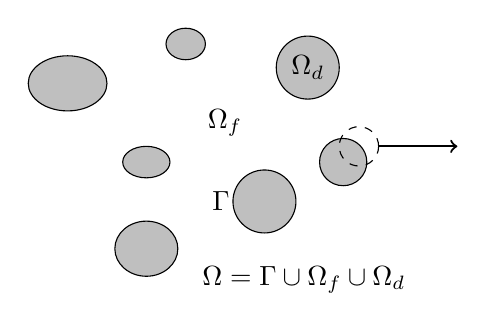
\begin{tikzpicture}
        \foreach \x/\y/\ra/\r in {
        1/3/0.2/0.25,
        2.55/2.7/0.4/0.4,
        0.5/0.4/0.35/0.4,
        2/1/0.4/0.4,
        3/1.5/0.3/0.3,
        0.5/1.5/0.2/0.3,
        -0.5/2.5/0.35/0.5}{
            \draw[fill=gray!50](\x,\y) ellipse(\r cm and \ra cm);
        }
        \draw[dashed](3.2,1.7)circle(0.25);
        % \draw[thick,->](3.2,1.7)++(0.1767,0.1767)--++(0.4,0.4)--++(1,0);
        \draw[thick,->](3.2,1.7)++(0.25,0)--++(1,0);
        \draw(2.55,2.7)node{$\Omega_d$};
        \draw(1.5,2)node{$\Omega_f$};
        \draw(1.45,1)node{$\Gamma$};
        \draw(2.5,0)node{$\Omega = \Gamma \cup \Omega_f \cup \Omega_d$};
        % \draw(2.5,-1)node{$\Gamma = \sum_\alpha \Gamma_\alpha$};
        % \draw(2.5,-0.5)node{$\Omega_2 = \sum_\alpha \Omega_\alpha$};
    \end{tikzpicture}
    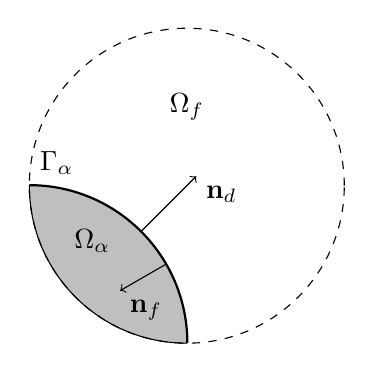
\begin{tikzpicture}%[scale = 0.9]
        \draw[very thick](0:2)arc(0:90:2)node[above right]{$\Gamma_\alpha$};
        \draw[fill=gray!50](0:2)arc(0:90:2)arc(180:270:2);
        \draw[dashed](2,2)circle(2);
        \draw[->](1.42,1.42)--++(0.7,0.7)node[below right]{$\textbf{n}_d$};
        \draw[->](1.73,1)--++(-0.577,-0.333)node[below right]{$\textbf{n}_f$};
        \draw(2,3)node{$\Omega_f$};
        \draw(0.8,1.3)node{$\Omega_\alpha$};
    \end{tikzpicture}
    \caption{Topology of dispersed two-phase flows.}%Domain definitions and scheme of the topology of dispersed two-phase flows.}
    \label{fig:Scheme}
\end{figure}

We consider a system consisting of two phases, separated by a sharp interface $\Gamma(t,\FF)$,
where $t$ represents the current time and $\FF$ an initial flow configuration. 
More detail will be given later regarding the meaning of what we call the initial \textit{flow configuration}. 
For now just think of it as a way to denote the dependence of the local functions such as $\Gamma(t,\FF)$ on the exact flow configuration. 
In opposition to the averaged fields introduced in \ref{sec:avg_def} which will be defined as the average of these local functions over all the configurations $\FF$. 
Each phase subdomain is denoted as $\Omega_f(t,\FF)$ and $\Omega_d(t,\FF)$, representing the continuous or fluid phase ($f$) and the dispersed phase ($d$), respectively (refer to Figure \ref{fig:Scheme}).
The entire domain, denoted as $\Omega$, is defined as the union of $\Omega_f$, $\Omega_d$, and $\Gamma$.
To track the position of the phase indexed $k$ and the interfaces, we introduce the phase indicator function $\chi_k$ defined as
\begin{align}
    \chi_k(\textbf{x},t,\FF) =  \left\{
      \begin{tabular}{cc}
        $1 \;\text{if} \;\textbf{x} \in \Omega_k(t,\FF)$\\
        $0 \;\text{if} \;\textbf{x} \notin \Omega_k(t,\FF)$
      \end{tabular}
      \right.
      \text{for $k = f,d$}.
      \label{eq:PIF}
\end{align}
Additionally, we define $\Omega_\alpha(t,\FF)$ as the domain delimited by the volume occupied by the particle labelled $\alpha$ at time $t$ and in the configuration $\FF$ (see \ref{fig:Scheme}). 
The union of each $\Omega_\alpha(t,\FF)$ for $\alpha = 1,\ldots N$, assuming $N$ particles are present in the flow, is equivalent to $\Omega_d(t,\FF)$.
Likewise, we suppose that $\Gamma(t,\FF)$ can be subdivided into $N$ subdomains denoted $\Gamma_\alpha(t,\FF)$, each of which represents the surface of the particle $\alpha$. 

\subsection{Topological equations}
Using the distribution formalism, one may show that $\chi_k(\textbf{x},t,\FF)$ obeys the following relations \citep{drew1983mathematical,orlando2023evolution}. 
\begin{align}
    \pddt \chi_k
    + \textbf{u}_I^0 \cdot \grad \chi_k
    &= 0,
    \label{eq:dt_chi_k}\\
    \label{eq:grad_chi_k}
    \grad \chi_k
    &= - \delta_I \textbf{n}_k, 
\end{align}
where $\textbf{u}^0_I(\textbf{x},t,\FF)$ is the velocity of the interface and $\delta_I(\textbf{x},t,\FF)$ is the Dirac function localized on the interface, also called the interfacial indicator function.
Throughout this work we employ the subscript $_I$ to indicate any quantity inherently defined on the interfaces, such as $\textbf{u}_I^0(\textbf{x},t,\FF)$ and $\delta_I(\textbf{x},t,\FF)$. 
Furthermore, we use the superscript `` $^0$ '' on a field to indicate that it is defined at the local or microscopic level, which implies that it is a function of the flow configuration $\FF$, the position vector $\textbf{x}$, and the time $t$. 
Therefore, for clarity and ease of reading purposes, we omit these arguments for any local function denoted by a `` $^0$ '' (including $\delta_I$ and $\chi_k$) as it is implicitly referring to $\textbf{x},t$ and $\FF$.

To describe the evolution of $\delta_I$ we derive a first equation by taking the gradient of \ref{eq:dt_chi_k} and then applying the dot product of the resulting expression with $\textbf{n}_k$.
A second equation is obtained by taking the gradient of the trivial relation: $\delta_I = \delta_I \textbf{n}_k\cdot \textbf{n}_k$.
This yields \citep{morel2007surface,orlando2023evolution}, 
\begin{align}
    \pddt \delta_I
    + \div [\delta_I (\textbf{u}_I^0\cdot \textbf{n}) \textbf{n}]
    &= \delta_I (\textbf{u}_I^0 \cdot \textbf{n})(\div\textbf{n}),
    \label{eq:dt_delta_I}\\
    \grad\delta_I 
    &= \textbf{n}\cdot  \grad (\textbf{n} \delta_I) 
    \label{eq:grad_delta_I}
\end{align} 
Remark that to derive \ref{eq:dt_delta_I} and \ref{eq:grad_delta_I} we have utilized the relations $\textbf{n}_k\cdot \pddt\textbf{n}_k= \frac{1}{2}\pddt(\textbf{n}_k\cdot \textbf{n}_k) = 0$ and $\grad \textbf{n}_k \cdot \textbf{n}_k =\frac{1}{2} \grad(\textbf{n}_k\cdot \textbf{n}_k) = 0$. 
Furthermore, we did not specify the index of the normal $\textbf{n}$ in \ref{eq:dt_delta_I} and \ref{eq:grad_delta_I} to highlight that both equations are independent of the index $k$. 
This is because \textbf{n} appears twice in each term of \ref{eq:dt_delta_I} and \ref{eq:grad_delta_I}.
Additionally, note that in \ref{eq:dt_delta_I} only the normal component of the surface velocity is present and that the term $\div \textbf{n}$ represents twice the mean curvature of the surface \citep{aris2012vectors}. 

\ref{eq:dt_chi_k}, \ref{eq:dt_delta_I}, \ref{eq:grad_delta_I} and \ref{eq:grad_chi_k} are commonly referred to as the topological equations of two-phase flows.
It describes the evolution in space and time of the topology of the flow interfaces.

\subsection{Local conservation equations}
\label{sec:local_eq}
Let now introduce the local conservation laws that govern the fluid inside bulk phases (inside $\Omega_d$ and $\Omega_f$) and on the interfaces (on $\Gamma$). 

\subsubsection{Inside the volumes}

Within phase $k$, we note $\rho_k^0$ the density, $\textbf{u}_k^0$ the local velocity and $E_k^0$ the local total energy per unit of mass.
All over the domain $\Omega_k$ the mass, momentum and total energy obey these conservation laws:
\begin{align}
    \label{eq:dt_rho}
    \pddt \rho_k^0  
    + \div (
        \rho_k^0\textbf{u}_k^0
    )
    &= 
    0,\\
    \label{eq:dt_rhou_k}
    \pddt (\rho_k^0\textbf{u}_k^0)  
    + \div (
        \rho_k^0\textbf{u}_k^0\textbf{u}_k^0
        - \bm{\sigma}_k^0 
    )
    &= 
    \rho_k^0 \textbf{g},\\
    \label{eq:dt_rhoE_k}
    \pddt (\rho_k^0E_k^0)  
    + \div (
        \rho_k^0E_k^0\textbf{u}_k^0
        + \textbf{q}_k^0
        - \textbf{u}_k^0 \cdot \bm{\sigma}_k^0 
        )
    &= 
    \textbf{u}_k^0 \cdot \textbf{g}  \rho_k^0, 
\end{align} 
respectively. 
Where $\bm\sigma_k^0$ and $\textbf{q}_k^0$ represent the stress tensor and the thermal energy flux of phase $k$, respectively. 
The vector $\textbf{g}$ is the acceleration of gravity which is the only body force considered here.
Additionally, the continuous phase is assumed Newtonian therefore, $\bm{\sigma}_f^0 = - p_f^0 \bm\delta + \mu_f \textbf{e}_f^0$, with $\textbf{e}_f^0 = \grad \textbf{u}_f^0+(\grad \textbf{u}_f^0)^\dagger$ the shear rate tensor, $\bm\delta$ the identity tensor and $p_f ^0$ the local pressure. 
No heat source will be considered in this study.

The total energy of phase $k$ can be further decomposed as $E_k^0 = e_k^0 + (u_k^0)^2/2$, where $e_k^0$ is the internal energy per unit of mass representing molecular agitation and $(u_k^0)^2/2$ is the kinetic energy per unit of mass.
This decomposition, along with the previous set of equations, leads us to two independent equations, one for $e_k^0$ and a second for $(u_k^0)^2/2$, they read
\begin{align}
    \label{eq:dt_rhou_k2}
    \pddt [\rho_k^0(u_k^0)^2]  
    + \div [\rho_k^0(u_k^0)^2\textbf{u}_k^0/2 - \textbf{u}_k^0 \cdot \bm{\sigma}_k^0]
    &=
    \rho_k^0\textbf{u}_2^0 \cdot \textbf{g}  
    -  \bm{\sigma}_k^0 : \grad \textbf{u}_k^0,
    \\
    \label{eq:dt_rhoe_k}
    \pddt (\rho_k^0e_k^0)  
    + \div (
        \rho_k^0e_k^0\textbf{u}_k^0
        + \textbf{q}_k^0
        )
    &= 
    \bm{\sigma}_k^0 : \grad \textbf{u}_k^0,
\end{align} 
respectively. 
We can observe that the term, $\bm{\sigma}_k^0 : \grad \textbf{u}_k^0$,  appears with opposite signs in \ref{eq:dt_rhou_k2} and \ref{eq:dt_rhoe_k}.
This indicates that the amount of energy transformed from kinetic to internal energy is given by $\bm{\sigma}_k^0 : \grad \textbf{u}_k^0$.
Thus, in the case of Newtonian fluids, $\bm{\sigma}_f^0 : \grad \textbf{u}_f^0$ represents the energy dissipation due to viscous forces, which then acts as a heat source in \ref{eq:dt_rhoe_k}. 

\subsubsection{On interfaces}

On the interface $\Gamma$ the governing equations take the form of $2D$ conservation laws. 
They are often viewed as \textit{jump conditions} or as boundary conditions for  \ref{eq:dt_rho}, \ref{eq:dt_rhou_k} and \ref{eq:dt_rhoE_k}. 
In the most general case, the mass, momentum and energy surface equations read as \citep{ishii2010thermo,morel2015mathematical,bothe2022sharp}, 
\begin{align}
    \label{eq:dt_rhoI}
    \pddt \rho_I^0
    + \divI (\rho_I^0\textbf{u}_{I}^0)
    + \rho_I^0 (\textbf{u}_I^0 \cdot \textbf{n})(\div \textbf{n})
    &= 
    -\Jump{
        \rho_k^0 (\textbf{u}_I - \textbf{u}_k)
    }
    \\
    \label{eq:dt_rhoIu_I}
    \pddt (\rho_I^0\textbf{u}_I^0)  
    + \divI (
        \rho_I^0\textbf{u}_{I}^0\textbf{u}_{I||}^0
        - \bm{\sigma}_{I||}^0)
        + \rho_I^0 \textbf{u}_I^0 (\textbf{u}_I^0 \cdot \textbf{n})(\div \textbf{n})
    &= 
    \rho_I^0 \textbf{g}
    - \Jump{
        \rho_k^0 \textbf{u}_k (\textbf{u}_I - \textbf{u}_k)
        + \bm\sigma^0_k
    }
    \\
    \label{eq:dt_rhoIE_I}
    \pddt (\rho_I^0E_I^0)  
    + \divI (
        \rho_I^0 E_I^0\textbf{u}_{I||}^0
        - \textbf{u}_I^0 \cdot \bm{\sigma}_{I||}^0 
        + \textbf{q}_{I||}^0
        )
    + \rho_I^0E_I^0  (\textbf{u}_I \cdot \textbf{n})(\div \textbf{n})
    &= 
    \textbf{u}_I^0 \cdot \textbf{g}  \rho_I^0 \nonumber\\
    &- \Jump{\textbf{u}_k^0 \cdot \bm{\sigma}_k^0 - \textbf{q}_k^0
    + \rho_k^0 E_k (\textbf{u}_I - \textbf{u}_k)
    },
\end{align} 
respectively.
Where $\rho_I^0$ is the interface density, $\rho_I^0\textbf{u}_I^0$ the interface momentum 
and $E_I^0 = e_I^0 + \frac{1}{2}(u_I^0)^2$ the total energy of the interface, with $e_I^0$ the internal energy of the interface.
$\bm{\sigma}_{I||}^0$ and $\textbf{q}_{I||}^0$ denote the momentum and heat fluxes on the interface, respectively.
Note that we use the subscript  $_{||}$ to indicate the projection of a field onto the plane tangential to the surface $\Gamma$. 
Specifically, for an arbitrary quantity $\textbf{f}$ defined on $\Gamma$, we denote its tangential projection as $\textbf{f}_{||} = (\bm\delta-\textbf{nn})\cdot \textbf{f}$. 
Thus, notice that the diffusive flux $\bm{\sigma}_{I||}^0$ in \ref{eq:dt_rhoIu_I} and \ref{eq:dt_rhoIE_I} is a quantity projected onto the tangential plane of $\Gamma$.
This arises from the fact that at thermodynamic equilibrium the diffusive flux $\bm{\sigma}_{I||}^0$ exhibits solely tangential components.
Specifically, we can write \citep{nadim1996concise,bothe2022sharp}
\begin{equation}
    \bm\sigma_{I||}^0 = \left[\gamma + (\mu_{Id} -\mu_{Is}) \divI\textbf{u}_I^0\right] \bm\delta_{||}
    +  \mu_{Is} \bm\delta_{||} \left[\grad_I\textbf{u}_I^0 + (\gradI \textbf{u}_I^0)^\dagger\right] \bm\delta_{||},
    \label{eq:surface_fluxes}
\end{equation}
where $\mu_{Id}$ and $\mu_{Is}$ are the interfaces dilatational and shear viscosities, respectively, and $\gamma$ is the surface tension coefficient. 
This observation holds significant implications for later analysis.

The previous definition also applies to the divergence operator, meaning that $\gradI= (\bm\delta-\textbf{nn})\cdot \grad$ is referred to as the surface divergence operator. 
Consequently, the flux terms of the form $\divI[(\ldots)_{||}]$ in \ref{eq:dt_rhoI}, \ref{eq:dt_rhoIu_I} and \ref{eq:dt_rhoIE_I} represent 2D diffusive and convective fluxes that result from tangential motions or diffusive processes at the interface. 
Conversely, the terms involving the local curvature $(\div \textbf{n})$ are related to the interface expansion or contraction resulting from the normal velocity of the interface $\textbf{u}_I^0\cdot \textbf{n}$. 
Thus, the latter term is the consequence of the time-varying metric of the interface, while the former can be non-zero for a static interface $\Gamma$. 
We introduced the notation $\Jump{\ldots}$, where $\Jump{\ldots} = \sum_{k=1}^2 [\ldots] \cdot \textbf{n}_k$ signifying the discontinuity across the interface.
Consequently, the terms present on the right-hand side of \ref{eq:dt_rhoI}, \ref{eq:dt_rhoIu_I} and \ref{eq:dt_rhoIE_I} represent the source due to the discontinuity of the bulk properties at each sides of the interface. 
Specifically, we recognize the terms related to mass transfer as $\rho_k^0 (\ldots) (\textbf{u}_I - \textbf{u}_k)$ where $(\ldots)$ refers to the quantity to be conserved. 


In \ref{ap:hypothesis} we expose the surface conservation equations considering no surface properties except the uniform surface tension effects, i.e. first term of \ref{eq:surface_fluxes} with $\gamma$ constant. 
This yields a much simpler set of equations for the interfaces that will be used in the last section of the present paper (see \ref{sec:application}). 
For further insights into the modeling of sharp interface thermodynamics a comprehensive review may be found in \cite{bothe2022sharp}. 

\subsubsection{Generic formulation}

For ease of understanding, we now introduce generic conservation laws in the volumes and on the interfaces. 
Let $f_k^0$ denote a volumetric quantity of arbitrary tensorial order defined in $\Omega_k$.
Likewise, let $f_I^0$ represent an arbitrary surface property defined on $\Gamma$.
Using the strategy outlined in \citep{ishii2010thermo,bothe2022sharp}, the local conservation equations for $f_k^0$ and $f_I^0$ yield,  
\begin{align}
    \label{eq:dt_f_k}
    \pddt f_k^0
    +\div \left(
        f_k^0\textbf{u}_k^0
        - \mathbf{\Phi}_k^0
        \right)
    &= 
    s_k^0
    & \text{ in } \Omega_k,&\\
    \pddt f_I^0 
    + f_I^0 (\textbf{u}_I \cdot \textbf{n})(\div \textbf{n})
    +\divI
    (f_I^0 \textbf{u}_{I||}^0
        - \mathbf{\Phi}_{I||}^0 )
    &= 
    s_I^0
    - \Jump{
       f_k (\textbf{u}_I^0 - \textbf{u}_k^0)
       + \mathbf{\Phi}_k^0
    } 
    & \text{ on } \Gamma,&
    \label{eq:dt_f_I}
\end{align}
respectively.
The tensors $\mathbf{\Phi}_k^0(f_k^0)$ and $\mathbf{\Phi}_{I||}^0(f_I^0)$ represent the non-convective fluxes corresponding to the quantities $f_k^0$ and $f_I^0$, respectively. 
Notice that $\mathbf{\Phi}_{I||}^0$ also carries the $_{||}$ subscript which implies that only the tangential component of this tensor plays a role in the surface balance equation. 
Similarly, $s_k^0(f_k^0)$ and $s_I^0(f_I^0)$ are the source terms corresponding to the quantities $f_k^0$ and $f_I^0$, respectively.
For practical uses, note that the advecting term in \ref{eq:dt_f_I} can be written in the more compact form $\divI(f_I^0 \textbf{u}_I^0)$. 
Indeed, one can show that $f_I^0 (\textbf{u}_I \cdot \textbf{n})(\div \textbf{n})
+\divI(f_I^0 \textbf{u}_{I||}^0) = \divI(f_I^0 \textbf{u}_I^0)$, by noticing that $\textbf{n}\cdot\gradI(\ldots) = 0$ and $\divI\textbf{n} = \div\textbf{n}$ \citep{nadim1996concise}.
It is important to note that \ref{eq:dt_f_k} and \ref{eq:dt_f_I} are defined uniquely in the domains $\Omega_k$ and $\Gamma$, respectively.
Consequently, these equations are referred to as local conservation equations. 


\subsection{The two-fluid formulation}
The presence function $\chi_k$, and the Dirac delta function $\delta_I$, allow the extension of \ref{eq:dt_f_k} and \ref{eq:dt_f_I} to the entire flow domain $\Omega$. 
This extension is achieved by employing the methodology introduced by \citet{drew1983mathematical} and \citet{kataoka1986local} for the conserving laws inside the volume (\ref{eq:dt_f_k}).
The two-fluid formulation may be obtained by multiplying \ref{eq:dt_f_k} by $\chi_k$. 
Using \ref{eq:dt_chi_k} and \ref{eq:grad_chi_k} we obtain
\begin{equation}
    \pddt (\chi_k f_k^0)
    + \div (
        \chi_k f_k^0 \textbf{u}_k^0
        - \chi_k \mathbf{\Phi}_k^0 
        )
    = 
    \chi_k s_k^0
    + \delta_I\left[
        f_k^0
        \left(
            \textbf{u}_I^0
            - \textbf{u}_k^0
        \right)
        + \mathbf{\Phi}_k^0
    \right]
    \cdot \textbf{n}_k.
    \label{eq:dt_chi_k_f_k}
\end{equation}
This yields an equation defined over $\Omega$, to be solved for the quantity $\chi_k f_k^0$ instead of $f_k^0$. 
Moreover, in contrast to \ref{eq:dt_f_k} we observe the emergence of the interfacial term $ \delta_I[\ldots]$ on the right-hand side of \ref{eq:dt_chi_k_f_k}. 

Likewise, multiplying \ref{eq:dt_f_I} by $\delta_I$ and making use of the topological equations (\ref{eq:dt_delta_I} and \ref{eq:grad_delta_I}) gives,
\begin{equation}
    \pddt (\delta_If_I^0)  
    + \div (
        \delta_I f_I^0 \textbf{u}_I^0
        - \delta_I \mathbf{\Phi}_{I||}^0 
        )
    = 
    \delta_Is_I^0
    - \delta_I\Jump{
    f_k^0 (\textbf{u}_I^0 - \textbf{u}_k^0)
    + \mathbf{\Phi}_k^0},
    \label{eq:dt_delta_I_f_I}
\end{equation}
which corresponds to the conservation equation of $\delta_If_I^0$, which is defined over $\Omega$.
As the derivation of \ref{eq:dt_delta_I_f_I} is not straightforward we provide intermediate steps in \ref{ap:interface_proof}. 
Although \ref{eq:dt_f_I} and \ref{eq:dt_delta_I_f_I} appear similar in many respects, they possess a fundamental distinction: \ref{eq:dt_f_I} is defined exclusively on $\Gamma$, it is a two-dimensional partial differential equation with a time-dependent metric, whereas \ref{eq:dt_delta_I_f_I} is a three-dimensional partial differential equation. 
This distinction holds significant importance, as the formulation of \ref{eq:dt_delta_I_f_I} proves to be more practical for numerical methods \citep{scorsim2021particle}. 
The set of equations formed by \ref{eq:dt_chi_k_f_k} for $k = f,d$ and the surface transport equation or \textit{jump condition} (\ref{eq:dt_delta_I_f_I}) is commonly known as the \textit{two-fluid} formulation of multiphase flows \citep{morel2015mathematical,tryggvason2011direct,drew1983mathematical,kataoka1986local}. 

Let us define a \textit{bulk} property $f^0$ as $f^0 = \sum_{k} \chi_k f_k^0 + \delta_I f_I^0$ where $f^0$ represents any property of the flow of arbitrary tensorial order.
Then by summing \ref{eq:dt_chi_k_f_k} for $k=f,d$ and \ref{eq:dt_delta_I_f_I}, one obtain the \textit{single-fluid} formulation of multiphase flows, namely,
\begin{equation}
   \pddt f^0
   + \div (
       f^0 \textbf{u}^0
       -  \mathbf{\Phi}^0 
    )
   = s^0. 
   \label{eq:dt_f}
\end{equation}
It should be noted that in the literature we rather define the \textit{bulk} quantities as $f^0 = \sum_k \chi_k f_k^0$, while the interfacial components are treated as source terms in \ref{eq:dt_f} \citep{morel2015mathematical,tryggvason2011direct,drew1983mathematical}. 
Nevertheless, we want to point out here that our definition of $f^0$ yields a straightforward transport equation for $f^0$ thereby ensuring the consistency of the entire system of equations.



